\documentclass{beamer}
\usepackage[latin1]{inputenc}
\usepackage{graphicx}
\usepackage{amsmath}
\usepackage{verbatim}
\usepackage{listings}
\usepackage{color}
\usetheme{Frankfurt}

\def\Tiny{\fontsize{4pt}{4pt}\selectfont}

\begin{document}

\usebackgroundtemplate
{
\includegraphics[height=\paperheight,width=\paperwidth]{pic/esrf_crisp/esrf_crisp_default.jpeg}
}

\begin{frame}{CRISP 2nd annual meeting}
\begin{center}
The use of hardware virtualization in RASHPA
\end{center}
\end{frame}

\begin{frame}{Contents}
  \begin{itemize}
  \item RASHPA context reminder
  \item Device virtualization
  \item The VPCIE framework
  \end{itemize}
\end{frame}

\begin{frame}{Context - RASHPA reminder}
  \begin{center}
    \includegraphics[width=20mm]{pic/dv_reminder/main.jpeg}
  \end{center}
  \begin{tiny}
  RASHPA basic goal is to transfer \textbf{detector} memory contents into
  a \textbf{backend} for further processing, visualisation or storage. To
  do so, RASHPA relies on low level hardware and software components\\
  \begin{itemize}
  \item a data transport layer, currently PCI Express over cable
  \item a data transmission engine implemented on XILINX FPGA
  \item LINUX kernel device driver and userland software
  \end{itemize}
  \end{tiny}
\end{frame}

\begin{frame}{Context - RASHPA project issues}
  \begin{small}
  Still being prototyped
  \begin{itemize}
  \item how to simplify hardware software codesign ?
  \end{itemize}

  Aims at using multiple PCIE links. Yet, the first prototype is single link
  \begin{itemize}
  \item how to scale the prototype platform ?
  \end{itemize}

  Well positionned to interface with PCIE based accelerating technologies
  \begin{itemize}
  \item how to test unavailable (too recent or expensive) hardware ?
  \end{itemize}
  \end{small}
\end{frame}

\begin{frame}{Context - solution}
  \begin{center} Solution: \textbf{device virtualization} \end{center}
\end{frame}

\begin{frame}{Device virtualization - main idea}
  \begin{center}
    \includegraphics[width=45mm]{pic/dv_redirect/main.jpeg}
  \end{center}
  \begin{small}
    Applications on a \textbf{host} machine access hardware via interfaces. By
    \textbf{instrumenting} these interfaces, one can \textbf{redirect} the accesses
    to a software implementing the device. The device is said to be
    \textbf{virtualized}.
  \end{small}
\end{frame}

\begin{frame}{Device virtualization - hardware access redirection (0)}
  \begin{small}
  Virtualization assumes device accesses are made using a known interface
  \begin{itemize}
  \item software library API (system calls)
  \item memory mapped registers
  \item CPU specific instructions (in, out)
  \end{itemize}
  \end{small}
\end{frame}

\begin{frame}{Device virtualization - hardware access redirection (1)}
  \begin{small}
  The interface is then instrumented to redirect access to the virtual device
  \begin{itemize}
  \item software hooking (code instrumentation, library replacing)
  \item instruction emulation (QEMU)
  \item hardware traps (page protection)
  \item architecture support (INTEL VT)
  \item paravirtualization (XEN)
  \end{itemize}
  \end{small}
\end{frame}

\begin{frame}{Device virtualization - applications}
  Device virtualization example applications
  \begin{itemize}
  \item support: application running on unmaintained platform
  \item security: sandboxing, reverse engineering
  \item quality: debugging, fault injection
  \item testing: milkymist, zinq, android
  \end{itemize}
\end{frame}

\begin{frame}{VPCIE - goals}
  VPCIE, a Virtual PCIE framework made for RASHPA
  \begin{itemize}
  \item virtualize PCIE endpoints
  \item generic enough to fit other projects
  \item the backend software must run \textbf{without any modification}
  \item should be possible to use VHDL for device simulation
  \end{itemize}
\end{frame}

\begin{frame}{VPCIE - RASHPA possible setup (0)}
  \begin{center}
  \includegraphics[width=70mm]{pic/dv_vpcie/main.jpeg}
  \end{center}
\end{frame}

\begin{frame}{VPCIE - RASHPA possible setup (1)}
  \begin{center}
  \includegraphics[width=70mm]{pic/dv_rashpa/main.jpeg}
  \end{center}
\end{frame}

\begin{frame}{VPCIE - opensource building blocks}
  QEMU 
  \begin{itemize}
  \item http://wiki.qemu.org/Main\_Page
  \item architecture emulator (X86\_64, ARM ...)
  \item used to trap PCIE hardware accesses
  \end{itemize}
  GHDL
  \begin{itemize}
  \item http://ghdl.free.fr
  \item VHDL frontend for GCC
  \item used to implement device in VHDL
  \end{itemize}
\end{frame}

\begin{frame}{VPCIE - RASHPA backend}
  RASHPA backend is a full featured LINUX system
  \begin{itemize}
  \item runs in a QEMU virtual machine
  \item PCIE accesses are trapped and sent over TCP to the devices
  \item PCIE forwarder is available as a QEMU patch
  \end{itemize}
\end{frame}

\begin{frame}{VPCIE - RASHPA devices}
  RASHPA devices
  \begin{itemize}
  \item run as a LINUX processes
  \item can be implemented in C or VHDL
  \item can be duplicated at will
  \end{itemize}
\end{frame}

\begin{frame}{VPCIE - benefits}
  Hardware software codesign
  \begin{itemize}
  \item reduce development time
  \item no \textbf{modification} on the backend software (esp. driver)
  \item act as a stimuli generator for VHDL simulations
  \end{itemize}

  Platform scaling
  \begin{itemize}
  \item one PCIE endpoint per LINUX process
  \end{itemize}

  Investigate unavailable technologies
  \begin{itemize}
  \item NVM Express support for QEMU is available
  \end{itemize}
\end{frame}

\begin{frame}{VPCIE - availability}
  \begin{center}https://github.com/texane/vpcie\end{center}
\end{frame}

\begin{frame}{VPCIE - demo}
  \begin{center}demo\end{center}
\end{frame}

\end{document}
